Este capítulo apresenta os fundamentos teóricos que sustentam o desenvolvimento deste trabalho, bem como os principais estudos e iniciativas relacionadas ao tema. A Seção \ref{sec:mercado-financeiro} aborda o mercado financeiro brasileiro, com ênfase na atuação da CVM e sua função reguladora. A Seção \ref{sec:analises} discute as diferentes abordagens de análise para investimentos, com foco na análise fundamentalista. A Seção \ref{sec:computacional} descreve a modelagem dos dados e os processos de integração utilizados no projeto. Por fim, a Seção \ref{sec:estado-arte} apresenta trabalhos acadêmicos e iniciativas similares à proposta deste estudo, destacando seus principais diferenciais.

\section{Mercado financeiro} \label{sec:mercado-financeiro} % OK

O mercado financeiro é um sistema que engloba uma variedade de instituições, instrumentos e atividades relacionadas à gestão de recursos financeiros. Ele abrange diferentes segmentos, incluindo o mercado de capitais, o mercado monetário, o mercado cambial e o mercado de derivativos. O principal propósito do mercado financeiro é facilitar a alocação eficiente de recursos entre poupadores e investidores, fornecendo oportunidades de investimento e financiamento para empresas, governos e indivíduos \cite{teixeira:2019:mercado, damodaran:2012:investimentos}.

No Brasil, o mercado financeiro é composto pelos segmentos de mercado de capitais, mercado monetário, mercado de crédito, mercado de câmbio e mercado de derivativos. O mercado de capitais envolve a negociação de ações, debêntures e outros ativos mobiliários. Esse segmento é fundamental para o financiamento das empresas, permitindo que elas captem recursos por meio da emissão de títulos negociáveis no mercado financeiro \cite{reis:2021:negociacao}.

O mercado monetário é o espaço onde ocorrem operações de curto prazo entre instituições financeiras e o Banco Central. Essas operações têm como objetivo controlar a liquidez da economia e a taxa de juros, garantindo o equilíbrio do sistema financeiro \cite{deSouzaFigueiredo:2021:mercado}.

O mercado de crédito destina-se ao financiamento de empresas e pessoas físicas por meio de empréstimos e financiamentos bancários. Esse segmento é essencial para a dinamização da economia, permitindo investimentos e consumo a partir da concessão de crédito.

O mercado de câmbio é responsável pelas transações de compra e venda de moedas estrangeiras. Sua função principal é viabilizar o comércio internacional, investimentos estrangeiros e a gestão de reservas cambiais \cite{gois:2019:efeito}.

O mercado de derivativos compreende a negociação de contratos futuros, opções e \textit{swaps}, instrumentos utilizados para a gestão de riscos financeiros. Esse segmento permite que investidores e empresas se protejam contra variações adversas nos preços de ativos e taxas de juros \cite{figueiredo:2023:capacidade}.

Dentro do mercado financeiro, as ações representam uma das principais modalidades de investimento. Uma ação é uma fração do capital social de uma empresa, conferindo ao seu detentor a propriedade de uma parcela da empresa emissora. Ao adquirir ações, o investidor se torna um sócio da empresa e pode ter direito a participação nos lucros distribuídos e, em alguns casos, a voto nas assembleias de acionistas \cite{reis:2021:negociacao, gomes:2007:bolsa}.

A negociação de ações ocorre principalmente em bolsas de valores, como a B3 no Brasil, onde investidores podem comprar e vender ativos. O preço das ações é determinado pela oferta e demanda, ou seja, pela interação entre compradores e vendedores no mercado \cite{santander:2024:pregao}. Além disso, diversos fatores influenciam a valorização ou desvalorização dos papéis, como os resultados financeiros das empresas, a conjuntura econômica e eventos geopolíticos \cite{damodaran:2012:investimentos, attie:2013:bolsa}.

Duas instituições fundamentais nesse ecossistema são a B3 e a CVM. A B3 atua como principal plataforma de negociação de ativos financeiros, enquanto a CVM desempenha um papel regulador crucial, garantindo transparência e equidade no mercado de capitais \cite{cvm:2023:funcoes}.

Criada pela Lei nº 6.385/1976 \cite{brasil:1976:lei6385}, a CVM tem como principal missão proteger os investidores e garantir o funcionamento eficiente do mercado de capitais \cite{cvm:2009:informacao}. Entre suas principais atribuições estão \cite{cvm:2009:informacao, roberto:2023:papel}:

\begin{itemize}
	\item regulamentação da abertura de capital de empresas e suas obrigações com o mercado;
	\item supervisão de corretoras, bancos de investimento e outras instituições financeiras;
	\item fiscalização da negociação de ativos financeiros e combate a fraudes e manipulações de mercado;
	\item garantia da transparência e divulgação de informações pelas companhias de capital aberto.
\end{itemize}

A CVM exige que todas as empresas listadas na bolsa de valores publiquem periodicamente suas demonstrações financeiras e outros documentos essenciais, como balanços patrimoniais e informações sobre acionistas relevantes. Essa transparência fortalece a confiança dos investidores e contribui para a estabilidade e o crescimento do mercado financeiro brasileiro \cite{fgv:2024:transformacao}.

Dessa forma, a regulamentação e a supervisão do mercado financeiro brasileiro desempenham um papel essencial na proteção dos investidores e no desenvolvimento sustentável do setor \cite{figueiredo:2023:capacidade}.

Para garantir a ampla disponibilidade dessas informações, a CVM mantém uma base de dados acessível ao público por meio de seu portal eletrônico\footnote{\url{https://dados.cvm.gov.br}.}  e sistemas especializados, como o Sistema Empresas.NET e o CVMWeb. As empresas registradas são obrigadas a enviar seus documentos periodicamente, os quais são disponibilizados em diversos formatos, como PDF, XML e XBRL, permitindo tanto a consulta manual quanto a análise automatizada \cite{cvm:2009:informacao}. Essa estrutura facilita o acompanhamento do mercado por investidores, analistas e demais interessados, promovendo maior transparência e acesso à informação.

A base de dados da CVM inclui:

\begin{itemize}
	\item demonstrações financeiras padronizadas (DFPs);
	\item informes trimestrais (ITRs);
	\item relatórios de governança corporativa;
	\item documentos de ofertas públicas de ações (IPO);
	\item dados sobre fundos de investimento e gestores de ativos.
\end{itemize}

\section{Análises para investimento} \label{sec:analises}

A análise de investimentos busca avaliar oportunidades de alocação de capital, utilizando diferentes abordagens para identificar ativos com potencial de retorno \cite{liaw:2011:business}. Entre essas abordagens, destacam-se a análise técnica, a análise de sentimento, a análise quantitativa, a análise macroeconômica e a análise fundamentalista.  

A análise técnica baseia-se no estudo de padrões gráficos e estatísticos do histórico de preços dos ativos. Os analistas técnicos utilizam indicadores como médias móveis, bandas de Bollinger e índices de força relativa para identificar tendências e pontos de compra ou venda no mercado \cite{omane:2019:time}.  

A análise de sentimento considera o impacto de notícias, redes sociais e opiniões de investidores sobre os ativos financeiros. Essa abordagem busca medir o comportamento do mercado a partir da análise de textos, discursos e volumes de menções relacionadas a determinados ativos, utilizando técnicas de processamento de linguagem natural e aprendizado de máquina \cite{kearney:2014:textual}.  

A análise quantitativa utiliza modelos matemáticos e estatísticos para prever movimentos de mercado e identificar oportunidades de investimento. Esse método frequentemente emprega algoritmos computacionais, regressões estatísticas e aprendizado de máquina para encontrar correlações e padrões em grandes volumes de dados financeiros \cite{sahu:2023:overview}.  

A análise macroeconômica avalia fatores econômicos amplos, como inflação, Produto Interno Bruto (PIB), taxas de juros e política monetária. Essa abordagem busca compreender como variáveis macroeconômicas influenciam os mercados financeiros e os preços dos ativos, sendo fundamental para investidores institucionais e gestores de fundos \cite{claessens:2017:macroeconomic}.  

A análise fundamentalista foca nos fundamentos financeiros das empresas, examinando indicadores como receita, lucro, endividamento e governança corporativa. Esse método busca determinar o valor intrínseco de um ativo, comparando-o ao seu preço de mercado para identificar se está subvalorizado ou supervalorizado. No contexto deste estudo, a análise fundamentalista será o enfoque principal, dada sua relevância na avaliação detalhada do desempenho financeiro e estratégico das companhias.  


A análise fundamentalista investiga os dados financeiros e operacionais das empresas para determinar seu valor intrínseco \cite{mathew:2024:overview}. Para isso, utiliza diversos indicadores que auxiliam na avaliação do desempenho financeiro, da estrutura de capital e da liquidez da empresa. Esses indicadores podem ser agrupados em quatro categorias principais: indicadores de rentabilidade, indicadores de liquidez, indicadores de endividamento e valor intrínseco.

\subsection{Indicadores de rentabilidade}

Os indicadores de rentabilidade medem a eficiência da empresa em gerar lucros em relação a diferentes bases financeiras. Esses cálculos são amplamente utilizados em estudos financeiros e derivam da contabilidade gerencial e da análise de demonstrações financeiras \cite{kothari:2001:capital}.

O lucro por ação (LPA) indica o montante de lucro líquido atribuído a cada ação ordinária em circulação da empresa. É um indicador essencial para avaliar o desempenho das ações no mercado.  
A fórmula é dada pela Equação \eqref{eq:lpa}. Considerando um lucro líquido de R\$ 10 milhões e 2 milhões de ações em circulação, tem-se o LPA de R\$ 5,00, conforme a Equação \eqref{eq:lpa-exemplo} \cite{omane:2019:time}.

\bigskip
\begin{subequations} \noindent
\begin{minipage}[b]{0.48\linewidth}
  \begin{equation} \label{eq:lpa}
    \text{LPA} = \frac{\text{Lucro líquido}}{\text{Número de ações}}
  \end{equation}
\end{minipage}
\hfill
\begin{minipage}[b]{0.48\linewidth}
  \begin{equation} \label{eq:lpa-exemplo}
    \text{LPA} = \frac{\numprint{10000000.00}}{\numprint{2000000.00}} = \numprint{5.00}
  \end{equation}
\end{minipage}
\end{subequations}
\bigskip

O índice preço por lucro (P/L) mede quanto os investidores estão dispostos a pagar pelo lucro da empresa.  
A fórmula está na Equação \eqref{eq:pl}. Se uma ação custa R\$ \numprint{50.00} e o LPA é R\$ \numprint{5.00}, o P/L será \numprint{10.00}, indicando que os investidores estão dispostos a pagar 10 vezes o lucro anual por ação \cite{sahu:2023:overview}.

\bigskip
\begin{subequations} \noindent
\begin{minipage}[b]{0.48\linewidth}
    \begin{equation} \label{eq:pl}
        \text{P/L} = \frac{\text{Preço da ação}}{\text{LPA}}
    \end{equation}
\end{minipage}
\hfill
\begin{minipage}[b]{0.48\linewidth}
    \begin{equation} \label{eq:pl-exemplo}
        \text{P/L} = \frac{\numprint{50.00}}{\numprint{5.00}} = \numprint{10.00}
    \end{equation}
\end{minipage}
\end{subequations}
\bigskip

O \textit{dividend yield} (DY) mede a rentabilidade dos dividendos pagos em relação ao preço da ação. Se a empresa paga R\$~\numprint{2.00} de dividendos por ação e o preço da ação é R\$~\numprint{40.00}, o cálculo da Equação~\eqref{eq:dy-exemplo} resulta em um DY de \numprint{5.00}\% \cite{kearney:2014:textual}.

\bigskip
\begin{subequations} \noindent
\begin{minipage}[b]{0.48\linewidth}
    \begin{equation} \label{eq:dy}
        \text{DY} = \frac{\text{Dividendo por ação}}{\text{Preço da ação}} \times 100
    \end{equation}
\end{minipage}
\hfill
\begin{minipage}[b]{0.48\linewidth}
    \begin{equation} \label{eq:dy-exemplo}
        \text{DY} = \frac{\numprint{2.00}}{\numprint{40.00}} \times 100 = \numprint{5.00}\%
    \end{equation}
\end{minipage}
\end{subequations}
\bigskip

\subsection{Indicadores de Liquidez}

Os indicadores de liquidez avaliam a capacidade da empresa de honrar suas obrigações de curto prazo \cite{claessens:2017:macroeconomic}. A Liquidez Corrente (LC) é expressa na Equação~\eqref{eq:lc}. Se o ativo circulante é de R\$~\numprint{500000} e o passivo circulante de R\$~\numprint{250000}, a liquidez corrente é igual a \numprint{2.00}, conforme a Equação~\eqref{eq:lc-exemplo}.

\bigskip
\begin{subequations} \noindent
\begin{minipage}[b]{0.48\linewidth}
    \begin{equation} \label{eq:lc}
        \text{LC} = \frac{\text{Ativo circulante}}{\text{Passivo circulante}}
    \end{equation}
\end{minipage}
\hfill
\begin{minipage}[b]{0.48\linewidth}
    \begin{equation}\label{eq:lc-exemplo}
        \text{LC} = \frac{\numprint{500000}}{\numprint{250000}} = \numprint{2.00}
    \end{equation}
\end{minipage}
\end{subequations}
\bigskip

\subsection{Indicadores de Endividamento}

Os indicadores de endividamento mostram a dependência da empresa em relação ao capital de terceiros \cite{kothari:2001:capital}. 

Um dos principais indicadores é a dívida bruta, que representa a soma do passivo circulante e do passivo não circulante da empresa, conforme definido na Equação~\eqref{eq:db}. A Equação~\eqref{eq:db} expressa a fórmula geral da dívida bruta, que é composta pelos valores de obrigações de curto prazo (passivo circulante) e de longo prazo (passivo não circulante). Já a Equação~\eqref{eq:db-exemplo} apresenta um exemplo numérico, onde a dívida bruta totaliza R\$~\numprint{3000000}, a partir da soma de R\$~\numprint{1000000} de passivo circulante e R\$~\numprint{2000000} de passivo não circulante.

\begin{subequations}
\begin{equation} \label{eq:db}
    \text{Dívida bruta} = \text{Passivo circulante} + \text{Passivo não circulante}
\end{equation}

\begin{equation} \label{eq:db-exemplo}
    \text{Dívida bruta} = \numprint{1000000} + \numprint{2000000} = \numprint{3000000}
\end{equation}
\end{subequations}

Por exemplo, se a dívida bruta é de R\$~\numprint{3000000} e o caixa e equivalentes de caixa totalizam R\$~\numprint{500000}, a dívida líquida será de R\$~\numprint{2500000}, conforme indicado na Equação~\eqref{eq:dl-exemplo}. A Equação~\eqref{eq:dl} define a dívida líquida, que representa o valor da dívida efetiva da empresa, descontado o montante disponível em caixa ou em aplicações de liquidez imediata. Já a Equação~\eqref{eq:dl-exemplo} ilustra esse conceito com valores hipotéticos, demonstrando que, ao subtrair R\$~\numprint{500000} disponíveis em caixa de uma dívida bruta de R\$~\numprint{3000000}, obtém-se uma dívida líquida de R\$~\numprint{2500000}.

\begin{subequations}
	\begin{equation} \label{eq:dl}
		\text{Dívida líquida} = \text{Dívida bruta} - \text{Caixa e equivalentes de caixa}
	\end{equation}
	\begin{equation} \label{eq:dl-exemplo}
		\text{Dívida líquida} = \numprint{3000000} - \numprint{500000} = \numprint{2500000}
	\end{equation}
\end{subequations}

\subsection{Valor intrínseco}

O valor intrínseco é estimado pelo método de Desconto de Fluxo de Caixa (DCF), conforme a Equação~\eqref{eq:vi}. Nessa equação, \( r \) representa a taxa de desconto e \( t \) o período de tempo. Com fluxo de caixa de R\$~\numprint{1000000} e taxa de desconto de \numprint{10}\%, o valor intrínseco resulta em R\$~\numprint{909090.91}, conforme demonstrado na Equação~\eqref{eq:vi-exemplo}. Esse cálculo reflete o valor presente do fluxo de caixa futuro \cite{figueiredo:2023:capacidade}.

\begin{subequations}
	\begin{equation} \label{eq:vi}
		\text{Valor intrínseco} = \sum \frac{\text{Fluxo de caixa esperado}}{(1 + r)^t}
	\end{equation}
	
	\begin{equation} \label{eq:vi-exemplo}
		\text{Valor intrínseco} = \frac{\numprint{1000000}}{(1 + \numprint{0.10})^1} = \frac{\numprint{1000000}}{\numprint{1.10}} = \numprint{909090.91}
	\end{equation}
\end{subequations}

\section{Modelagem e integração de dados} \label{sec:computacional}

A modelagem e integração de dados são etapas fundamentais para a construção de um sistema automatizado de análise fundamentalista. Neste trabalho, essas etapas têm o propósito de estruturar, consolidar e organizar os dados disponibilizados pela CVM, garantindo sua utilização eficiente e integrada. A seguir, são apresentadas as principais abordagens empregadas na modelagem dos dados, bem como os métodos utilizados para sua integração, assegurando a consistência, acessibilidade e interoperabilidade das informações no sistema desenvolvido.

\subsection{Modelagem dos dados e estruturação lógica}

A modelagem de dados é uma etapa fundamental no desenvolvimento de sistemas que manipulam grandes volumes de informações, especialmente em contextos financeiros, onde a integridade, consistência e escalabilidade são requisitos indispensáveis \cite{elmasri:2005:sistemas}. Neste trabalho, adotou-se uma abordagem centrada na modelagem lógica, com o objetivo de estruturar uma base de dados relacional robusta, capaz de integrar e armazenar dados públicos oriundos da CVM.

A modelagem lógica traduz os requisitos identificados no domínio do problema em uma estrutura formal que define, de maneira precisa, as tabelas, os atributos, os tipos de dados e as restrições de integridade necessárias para a representação das entidades envolvidas \cite{connolly:2015:database}. Diferente da modelagem conceitual, que geralmente se utiliza de representações como o Diagrama Entidade-Relacionamento (DER), a modelagem lógica já incorpora aspectos técnicos relacionados à implementação em um Sistema de Gerenciamento de Banco de Dados (SGBD), neste caso, o MySQL.

A Figura \ref{fig:esquema_logico} apresenta o esquema lógico elaborado com base em práticas de engenharia reversa e análise das documentações e estruturas disponibilizadas pela CVM. Essa técnica permite extrair o modelo de dados a partir de fontes existentes, facilitando o redesenho e a normalização da base de dados \cite{scannapieco:2006:data}.

\begin{figure}[!htb] 
	\centering
	\caption{Esquema lógico do banco de dados para integração de dados da CVM.} 
	\label{fig:esquema_logico}
	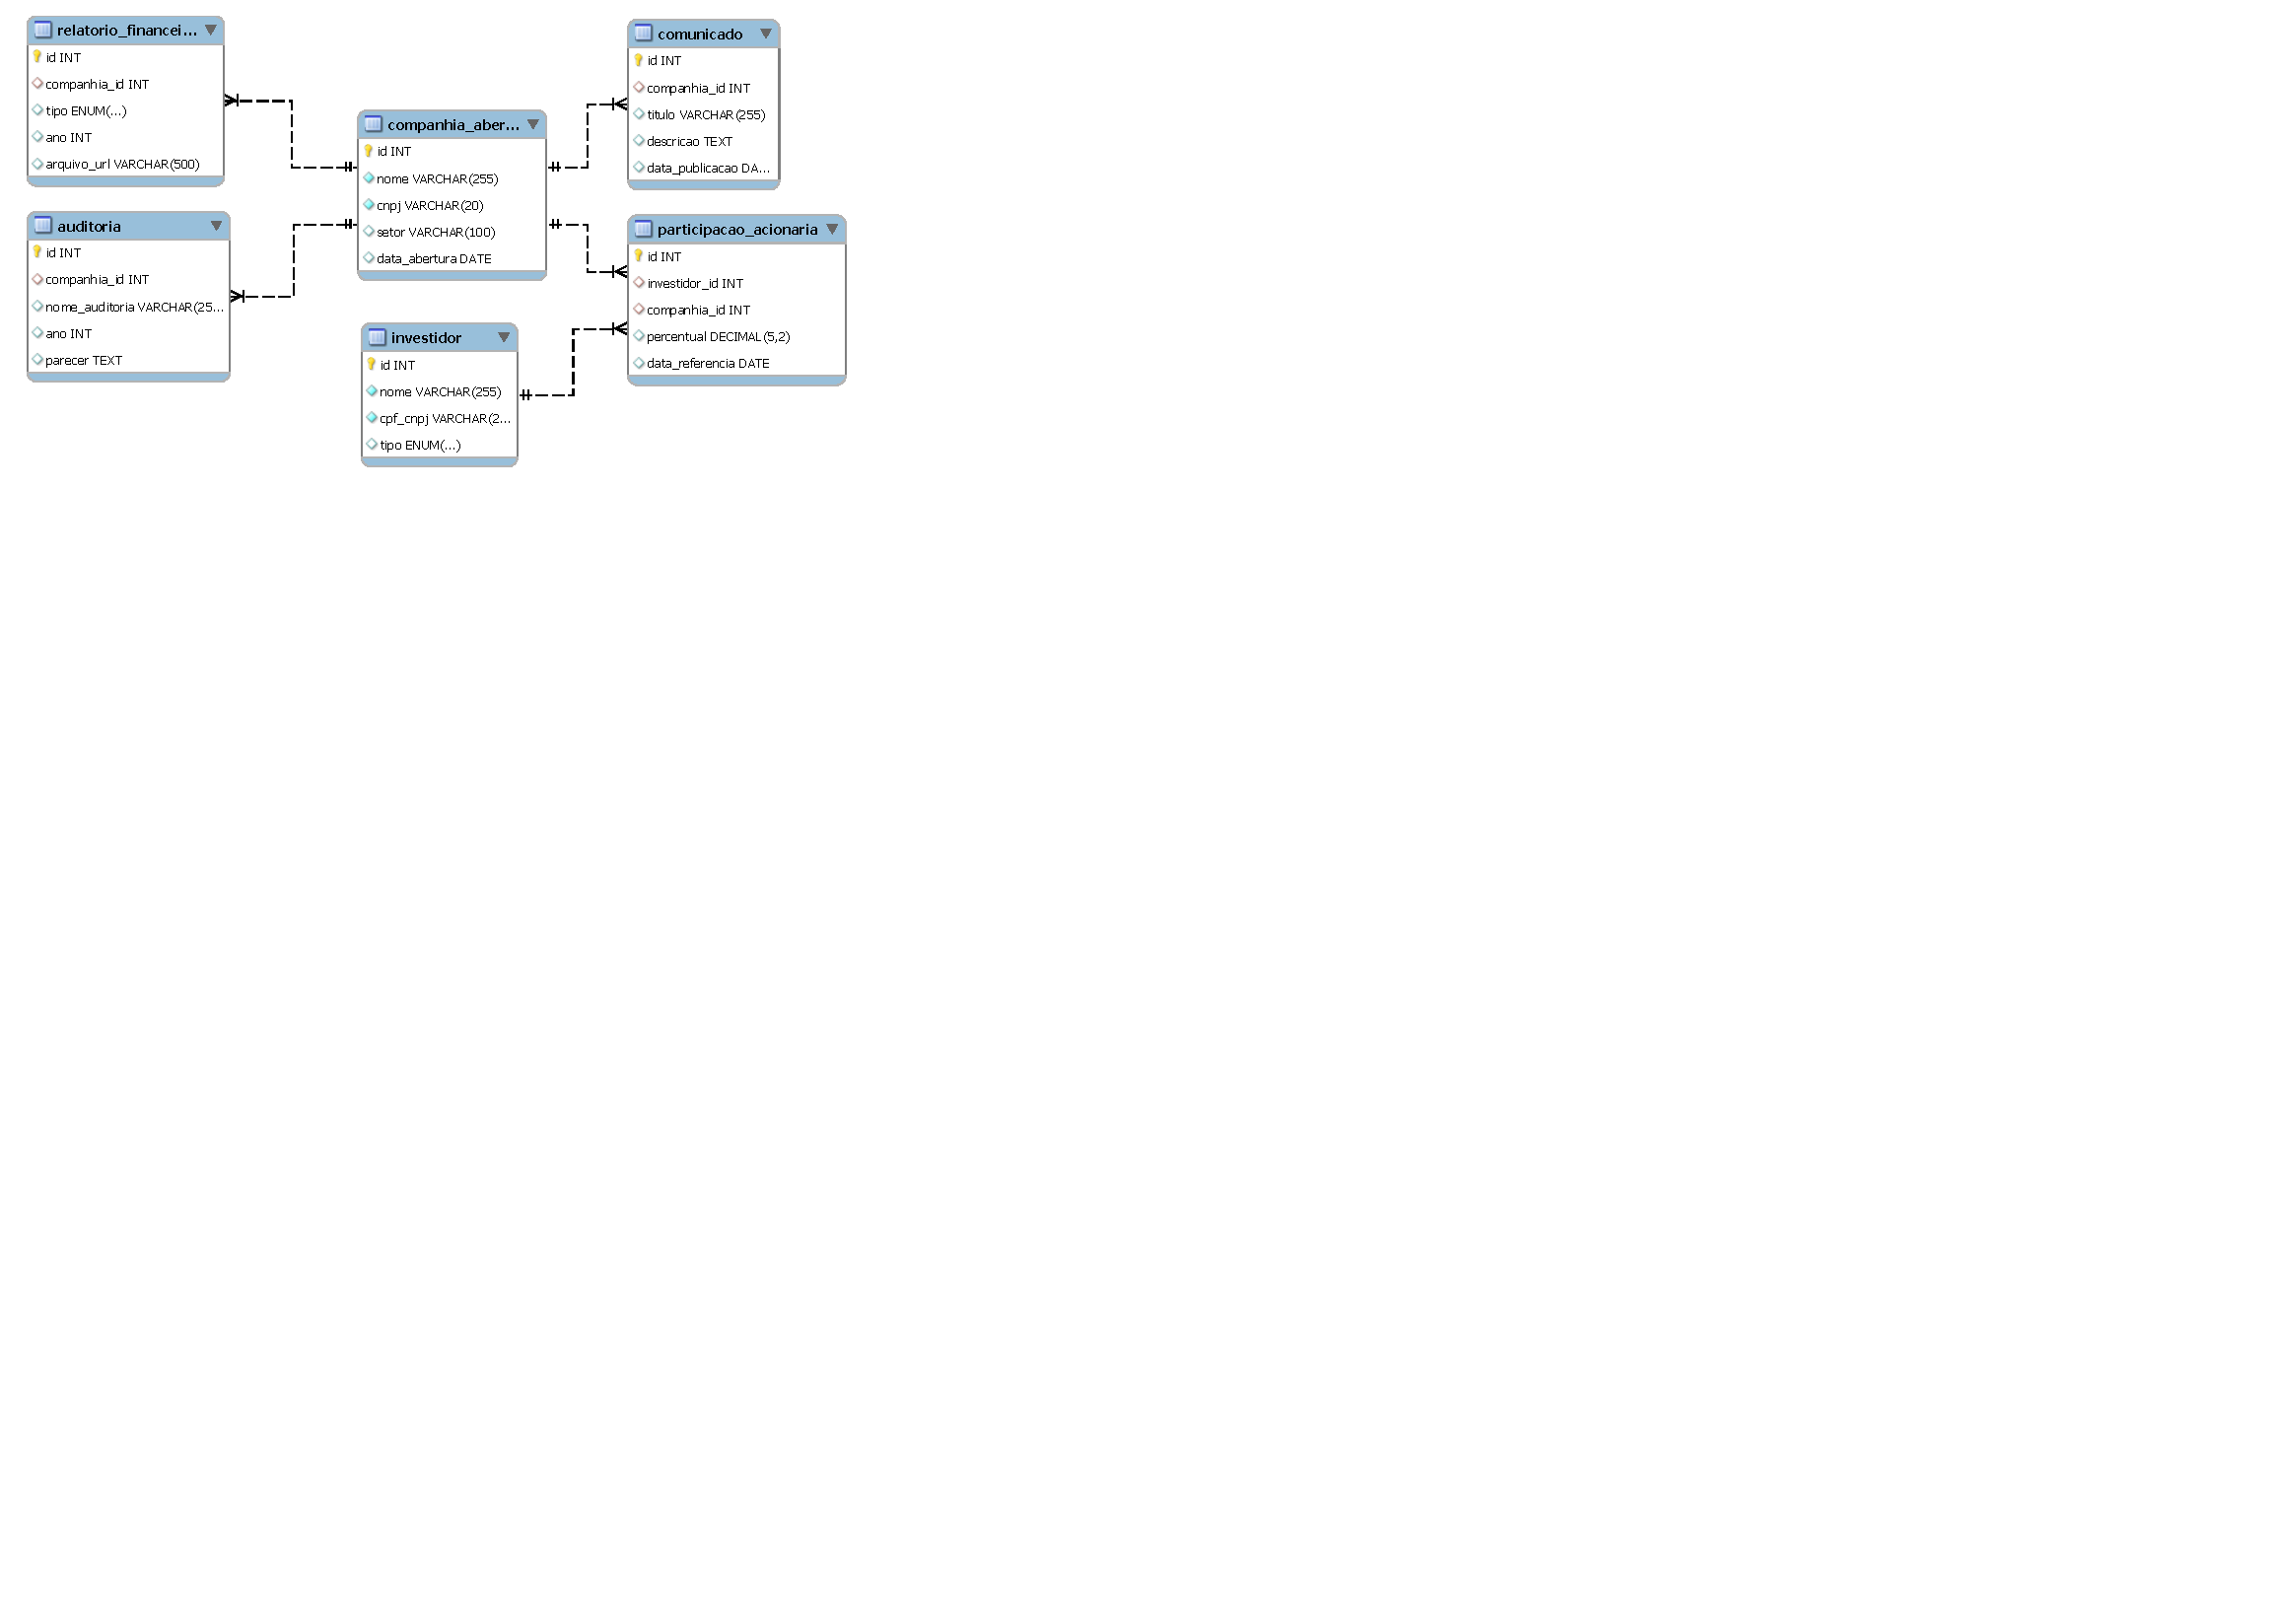
\includegraphics[width=0.9\textwidth]{figuras/esquema_logico.pdf}
	\vspace{1mm}
	\parbox[c]{0.9\textwidth}{\raggedright \legend{Elaborado pelo autor, 2024.}}
\end{figure}

O modelo proposto é composto pelas seguintes tabelas:

\begin{itemize}
	\item \textit{companhia\_aberta}
	\item \textit{comunicado}
	\item \textit{investidor}
	\item \textit{participacao\_acionaria}
	\item \textit{auditoria}
	\item \textit{relatorio\_financeiro}
\end{itemize}

A tabela \textit{companhia\_aberta} centraliza os dados cadastrais das empresas registradas na CVM, contendo atributos como \textit{nome}, \textit{cnpj}, \textit{setor} e \textit{data\_abertura}. O campo \textit{cnpj} possui uma restrição de unicidade (\textit{UNIQUE}) para garantir a integridade dos dados identificadores.

A tabela \textit{comunicado} armazena registros de publicações oficiais vinculadas às companhias, sendo referenciada pela chave estrangeira \textit{companhia\_id}, que estabelece uma relação com a tabela \textit{companhia\_aberta}. Esse vínculo viabiliza a rastreabilidade entre os comunicados e as empresas emissores.

A tabela \textit{investidor} registra os agentes que detêm participações acionárias, identificados pelo atributo \textit{cpf\_cnpj}, e categorizados segundo o tipo de investidor (\textit{Pessoa Física} ou \textit{Pessoa Jurídica}), utilizando a estrutura \textit{ENUM} para controle de domínio.

A tabela \textit{participacao\_acionaria} representa a associação entre investidores e companhias abertas, permitindo o registro da proporção de ações detidas por data de referência. Essa tabela possui chaves estrangeiras para as tabelas \textit{investidor} e \textit{companhia\_aberta}, o que possibilita a análise de composição societária ao longo do tempo.

A tabela \textit{auditoria} documenta os pareceres emitidos por empresas auditoras sobre as demonstrações financeiras das companhias, detalhando o ano do parecer, o nome da auditoria e a descrição do conteúdo emitido.

Por fim, a tabela \textit{relatorio\_financeiro} concentra os metadados dos arquivos financeiros disponibilizados pela CVM, como os Demonstrativos Financeiros Padronizados (DFP), Informações Trimestrais (ITR), o Formulário de Referência e o IAN. Cada registro inclui o tipo do documento, o ano de referência e o link para o arquivo original.

Essa estrutura relacional foi projetada visando à normalização dos dados, conforme as boas práticas de projeto de bancos de dados relacionais \cite{elmasri:2016:fundamentals}. A modelagem lógica aqui apresentada oferece a base necessária para uma integração eficiente e escalável, compatível com análises automatizadas de caráter fundamentalista. Sua implementação favorece a consistência da base de dados, o desempenho nas consultas SQL e a reutilização de componentes em diferentes módulos do sistema.



\subsection{Processo de integração de dados}

A integração de dados é um procedimento essencial que consolida informações oriundas de diversas fontes, garantindo consistência, qualidade e acessibilidade para análises estratégicas e operacionais. Esse processo transforma dados brutos em informações valiosas para a tomada de decisão e é composto por etapas interdependentes: extração, transformação e carga.

Na etapa de extração, os dados são coletados diretamente de múltiplas fontes, como os repositórios da CVM. Essa fase utiliza técnicas que asseguram a captura completa e precisa das informações, minimizando riscos de perda ou corrupção. No presente trabalho, essa etapa foi implementada por meio de \textit{scripts} automatizados em Python, que realizam o download de arquivos compactados disponibilizados pela CVM, como o \texttt{dfp\_cia\_aberta\_2022.zip}. O sistema verifica a existência prévia dos arquivos e sua integridade antes de prosseguir com o processamento, evitando redundâncias e falhas.

Após a extração, os dados brutos passam por um processo de transformação que envolve padronização, limpeza, normalização e aplicação de regras de negócio. Essa etapa é responsável por eliminar inconsistências, corrigir valores ausentes, ajustar formatos e estruturar os dados para análises mais sofisticadas. No contexto deste projeto, foram realizadas conversões de tipos, unificação de formatos de datas e remoção de duplicidades. Informações como o código da conta contábil (\texttt{CD\_CONTA}) foram associadas às suas descrições completas com base nos planos de contas divulgados pela CVM, garantindo maior legibilidade e utilidade analítica.

Na etapa final, os dados transformados são carregados em um banco de dados relacional estruturado, visando facilitar a manipulação, a consulta e a análise posterior. Para este trabalho, optou-se pelo uso do SQLite como solução leve e eficiente, adequada ao escopo local da ferramenta desenvolvida. As tabelas foram criadas respeitando normas de integridade referencial, com chaves primárias e estrangeiras bem definidas. Dados financeiros, cadastrais e operacionais foram organizados em tabelas como \texttt{demonstrativo\_financeiro}, \texttt{informacao\_trimestral} e \texttt{empresas}, possibilitando análises temporais, cálculo de indicadores como LPA e P/L, entre outros.

A integração harmônica dessas etapas resultou em uma base de dados confiável e atualizada, que sustenta a automatização dos processos analíticos e permite a construção de modelos quantitativos e preditivos. Essa abordagem se mostra fundamental para a aplicação da análise fundamentalista no contexto do mercado financeiro, proporcionando uma visão estruturada e estratégica para a tomada de decisão \cite{costa:2024:integraccao, halevy:2006:data}.

\section{Estado da arte} \label{sec:estado-arte}

Nesta seção, são analisados os principais estudos acadêmicos e projetos práticos que fundamentam a abordagem deste trabalho. Inicialmente, apresenta-se uma síntese dos trabalhos existentes, destacando seus objetivos, metodologias empregadas e limitações encontradas. Em seguida, evidencia-se como o presente estudo propõe uma integração inédita de dados e técnicas, superando as deficiências das abordagens anteriores.

\subsection{Trabalhos acadêmicos}

Os estudos acadêmicos voltados à modelagem e à análise de dados financeiros têm se concentrado na automatização da análise fundamentalista e na adaptação de modelos tradicionais ao contexto do mercado brasileiro. Por exemplo, \citet{montoia:2021:automatizaccao} desenvolvem um sistema automatizado para a análise de ações, enfatizando a melhoria na rapidez e na eficiência da tomada de decisões. Esse trabalho detalha a aplicação de algoritmos de processamento de dados que reduzem a intervenção manual, permitindo uma análise em tempo real dos indicadores financeiros.

De forma complementar, \citet{deAraujo:2021:modelo} propôs um modelo flexível que adapta os conceitos da análise fundamentalista para refletir as particularidades dos dados nacionais, considerando variáveis específicas do mercado brasileiro. Esse estudo destaca a importância da customização dos parâmetros e a integração de variáveis macroeconômicas na modelagem financeira.

Além disso, \citet{delalibera:2023:automatizaccao} aprimorou metodologias tradicionais, como o Modelo Rojo, para avaliação de ativos, enfatizando a precisão na quantificação de riscos e oportunidades de investimento. Este trabalho apresenta uma abordagem robusta que combina técnicas estatísticas com algoritmos de \textit{machine learning} para melhorar a acurácia das previsões. Por sua vez, \citet{reis:2020:analise} investigou a aplicação prática desses métodos na análise das ações negociadas, proporcionando \textit{insights} sobre a volatilidade do mercado e a relevância de diferentes indicadores financeiros.

Outros estudos, como o de \citet{vieira:2019:montagem}, analisam estratégias de montagem de carteiras de ações, comparando a performance das carteiras com índices de mercado e ressaltando as dificuldades na diversificação e no balanceamento dos ativos. Da mesma forma, \citet{freitas:2020:analise} explorou a aplicação criteriosa de indicadores no setor bancário, evidenciando os desafios em medir a solidez financeira e a eficiência operacional de instituições financeiras.

\subsection{Projetos e plataformas similares}

No campo dos projetos práticos, diversas iniciativas presentes em repositórios, especialmente no GitHub, vêm se destacando por oferecer ferramentas e bases de dados voltadas para a extração e análise de informações financeiras. Por exemplo, o projeto de \citet{paiva:2025:projetoGitHub} apresenta um sistema integrado que coleta, processa e organiza dados contábeis de empresas. Essa ferramenta tem como objetivo facilitar a aplicação da análise fundamentalista ao disponibilizar dados de forma estruturada e acessível, promovendo maior transparência e facilidade na análise dos balanços.

De maneira similar, \citet{minas:2025:projetoGitHub} propõe uma abordagem inovadora para a análise de balanços empresariais, enfatizando a importância da normalização dos dados e da criação de indicadores personalizados que se ajustem às especificidades de cada setor. Repositórios como os de \citet{fontinele:2025:projetoGitHub} e \citet{louredo:2025:projetoGitHub} se destacam ao desenvolver ferramentas específicas para interpretar demonstrações financeiras a partir de dados públicos, permitindo que o usuário identifique rapidamente pontos críticos e oportunidades de investimento. Contudo, grande parte dessas iniciativas se restringe à coleta e ao processamento dos dados, sem oferecer uma análise histórica contínua que possibilite a compreensão das tendências de longo prazo.

\subsection{Diferencial do trabalho proposto}

O diferencial do presente trabalho reside na integração de um histórico abrangente de dados financeiros com um sistema automatizado de acesso e análise das informações públicas disponibilizadas pela CVM. Embora os experimentos realizados tenham utilizado um recorte temporal de cinco anos, a ferramenta não se limita a esse intervalo. Enquanto a CVM mantiver a estrutura dos dados em seus repositórios, o sistema permanecerá funcional e poderá ser continuamente alimentado com novos dados, garantindo sua atualização e longevidade.

A proposta se distingue, ainda, por tratar-se de uma solução de código aberto, o que permite sua auditoria, personalização e extensão por outros pesquisadores e profissionais interessados. Essa abertura favorece a colaboração contínua, possibilitando o aprimoramento da ferramenta e sua adaptação a novos contextos analíticos ou setores econômicos específicos.

A abordagem adotada neste trabalho viabiliza tanto a avaliação contínua e comparativa dos dados quanto a análise contextualizada das informações. A avaliação contínua é sustentada pelo acúmulo de dados históricos, o que permite identificar tendências e padrões relevantes ao longo do tempo. Já a análise contextualizada emerge da capacidade de combinar dados históricos e atuais, ampliando a compreensão sobre ciclos econômicos, sazonalidades e eventos que impactam o mercado.

As principais inovações e contribuições do sistema desenvolvido podem ser resumidas nos seguintes pontos:

\begin{itemize}
	\item integração de dados históricos financeiros em larga escala;
	\item processamento automatizado, com foco em escalabilidade e reusabilidade;
	\item contextualização dos indicadores contábeis e financeiros;
	\item manutenção da funcionalidade do sistema diante de novas atualizações da CVM, desde que preservada a estrutura de dados;
	\item disponibilização em formato de código aberto, fomentando a transparência e a colaboração.
\end{itemize}

Ao superar as limitações de iniciativas anteriores, que se restringem majoritariamente à coleta e estruturação pontual dos dados, a solução apresentada promove uma abordagem sistemática e extensível, capaz de subsidiar análises fundamentalistas robustas e atualizadas. Essa característica torna o sistema especialmente útil para aplicações acadêmicas, institucionais e profissionais voltadas à tomada de decisão baseada em fundamentos econômicos e financeiros.